\documentclass{tietreport}

% ==================================================
% REQUIRED PACKAGES
% ==================================================
\usepackage{graphicx}
\usepackage{booktabs}
\usepackage{amsmath}
\usepackage{amssymb}
\usepackage{float}
\usepackage{tabularx}
\usepackage{caption}
\usepackage{xcolor}
\usepackage{colortbl}
\usepackage{array}
\usepackage{listings}

% ==================================================
% GRAPHICS PATH CONFIGURATION
% ==================================================
\graphicspath{{../diagram/}{../diagram/VR_Everywhere_UseCaseTemplate/}{./images/}{./}}

% ==================================================
% TIGHT FLOAT & SPACING CONTROLS (Eliminates Gaps)
% ==================================================
\raggedbottom
\setlength{\parindent}{0pt}
\setlength{\parskip}{4pt}

\setlength{\floatsep}{4pt plus 1pt minus 1pt}
\setlength{\textfloatsep}{6pt plus 1pt minus 1pt}
\setlength{\intextsep}{4pt plus 1pt minus 1pt}
\captionsetup{skip=4pt}

% Remove blank pages caused by two-sided cleardoublepage
\let\cleardoublepage\clearpage

% Hyperlink configuration
\usepackage{hyperref}
\hypersetup{
    hidelinks,
    colorlinks=false
}

% Bibliography configuration
\usepackage[
  date=year,
  style=alphabetic,
  backend=biber,
  sorting=nty,
  maxnames=5,
  minnames=3,
  maxalphanames=4,
  minalphanames=3,
  backref=true,
  doi=false,
  isbn=false,
  url=false,
  eprint=false
]{biblatex}
\addbibresource{references.bib}

% Custom table styling colors
\definecolor{tableheader}{RGB}{220, 235, 245}
\definecolor{tablealt}{RGB}{247, 250, 253}
\definecolor{ucboxblue}{RGB}{230, 244, 250}
\definecolor{ucboxgreen}{RGB}{232, 248, 235}
\definecolor{ucboxpurple}{RGB}{245, 236, 250}
\definecolor{ucboxorange}{RGB}{254, 243, 230}

%% ==================================================
%% PROJECT DETAILS & METADATA
%% ==================================================

\TitlePageHeader{%
  UCS503P - Software Engineering Project%
}

\ProjectTitle{%
  VR Everywhere: Virtual Travel Experience%
}

\ProjectSubTitle{%
  An Immersive Virtual Reality Platform for Accessible Cultural and Heritage Tourism%
}

\author{%
  \texttt{1024170428} Abhishek Garg \\
  \texttt{1024170432} Deepak \\
  \texttt{1024170436} Harnoor Kaur Dran%
}

\TitlePageSubText{%
  Group: \texttt{COPC} BE Third Year, CSE%
}

\AdvisorName{%
  Dr. Nisha Thakur%
}

\TitlePageFooterText{{%
    \large Final Evaluation \\[0.2cm]
    \bfseries Computer Science and Engineering Department%
  } \\[0.15cm]
  Thapar Institute of Engineering and Technology, Patiala%
}

%% ==================================================

\begin{document}

% Title page
\maketitle
\clearpage

% Table of contents
\tableofcontents
\clearpage

% ==================================================
% CHAPTER 1: INTRODUCTION
% ==================================================

\chapter{Introduction}

\section{Background and Context}

Travelling to world-renowned cultural, architectural, and historical destinations provides immense educational enrichment, cross-cultural appreciation, and personal inspiration. However, physical travel is frequently restricted or entirely precluded by substantial financial costs, long geographic distances, physical mobility constraints, health limitations, and demanding academic or professional schedules.

Traditional travel resources, encyclopedias, and educational websites typically present static two-dimensional photographs, brief text summaries, or passive promotional video clips. While informative, these media fail to deliver the visceral sensation of spatial scale, architectural depth, and personal agency required to genuinely appreciate global heritage monuments. Crucially, historical background, architectural trivia, interactive maps, and authentic soundscapes are scattered across disparate platforms rather than unified into an engaging exploratory medium.

Virtual Reality (VR) and Web-based 3D graphics (WebGL and WebXR) provide a transformative solution to these challenges. By synthesizing high-resolution 360-degree equirectangular environments, interactive 3D spatial points of interest, synchronized voice guides, and procedural ambient soundscapes, VR bridges the gap between physical absence and spatial presence. 

The \textbf{VR Everywhere} project engineers an accessible, responsive, and deployable virtual travel platform. The system empowers students, researchers, and armchair tourists to explore iconic cultural heritage sites worldwide—including the Taj Mahal, the Roman Colosseum, Machu Picchu, Fushimi Inari Taisha, and the Great Pyramids of Giza—directly from standard modern web browsers, mobile smartphones equipped with gyroscopic motion sensing, and low-cost stereoscopic VR Cardboard headsets without requiring costly proprietary hardware.

\subsection{Problem Statement}

Physical travel to distant heritage destinations remains inaccessible to wide demographics due to several critical constraints:

\begin{itemize}
  \item \textbf{Accessibility and Physical Limitations:} Individuals with mobility impairments, elderly citizens, and individuals with chronic medical conditions cannot physically navigate steep staircases, rocky paths, or high-altitude terrain (such as the rugged mountain steps of Machu Picchu).
  \item \textbf{Prohibitive Financial Costs:} International flights, transit logistics, lodging, visa fees, and tourist admissions impose substantial financial barriers, especially for students and budget-conscious learners.
  \item \textbf{Academic and Professional Time Constraints:} Rigid school, university, and workplace commitments rarely permit extended travel itineraries.
  \item \textbf{Fragmented and Static Information:} Historical facts, architectural significance, structural layout, and auditory ambiance are scattered across disparate websites, textbooks, and video repositories without an integrated, spatial learning environment.
  \item \textbf{Hardware and Platform Barriers in Existing VR Systems:} Most commercial virtual reality experiences require expensive dedicated headsets (e.g., Meta Quest, HTC Vive) and heavy local desktop installations, excluding smartphone and standard web users.
\end{itemize}

\section{Project Objectives}

The primary engineering goal of VR Everywhere is to design, develop, and evaluate an accessible, cross-platform virtual travel system with the following specific objectives:

\begin{enumerate}
  \item \textbf{Develop an End-to-End Virtual Travel Workflow:} Implement a fluid user journey spanning user registration, secure session authentication, destination catalog discovery, interactive 360-degree photosphere exploration, multi-waypoint navigation, and personalized favorites bookmarking.
  \item \textbf{Curate High-Fidelity Cultural Destinations:} Assemble rich architectural, historical, and geographical datasets for prominent global landmarks, including equirectangular panoramic photospheres, seasonal visit recommendations, and structural metadata.
  \item \textbf{Implement Interactive 3D Spatial Hotspots:} Project responsive 3D billboarded beacons within the virtual scenes using raycasting to surface curated cultural, historical, and architectural trivia upon user interaction.
  \item \textbf{Integrate Multi-Modal Audio Experiences:} Deliver dual-layer auditory guidance combining text-to-speech voice narration for architectural facts with procedural, synthesized ambient soundscapes (e.g., gentle breeze, flowing water, and temple chimes) using the Web Audio API.
  \item \textbf{Implement Street-View Waypoint Walking:} Support interactive traversal between connected vantage points (e.g., advancing from the Central Reflection Pool to the Grand Imperial Heritage Hall) with cinematic transitions, spatial footstep audio, and boundary limit protection.
  \item \textbf{Provide Mobile Gyroscope and Stereoscopic Headset VR:} Engineer dual-viewport stereoscopic rendering for mobile VR Cardboard viewers, integrating device orientation quaternion transforms to ensure stable, eye-level horizon tracking and pitch-clamping safeguards.
  \item \textbf{Ensure Robust User Account and State Persistence:} Provide user profile management, secure credential handling, password recovery, and cross-session persistence of explored tour histories and favorite destinations.
\end{enumerate}

% ==================================================
% CHAPTER 2: METHODOLOGY & DESIGN
% ==================================================

\chapter{Methodology and Design}

\section{System Architecture}

VR Everywhere is designed according to a modern, decoupled three-tier architectural model that separates the client presentation layer, the application business logic, and the persistent data layer. 

The presentation tier is implemented as a single-page web application using React 18, Vite, Three.js, and Tailwind CSS. It is responsible for rendering the 3D WebGL spherical canvas, managing camera orientation through mouse, touch, or device gyroscope sensors, handling audio synthesis, and presenting floating HUD overlays. 

The business logic tier coordinates user authentication, destination catalog queries, and session statistics. For local client-side deployment and offline capability, the system utilizes local storage caching and service-layer modules for credential validation and favorite bookmarking, while maintaining an extensible API contract compatible with a Spring Boot REST backend. 

The persistent data tier maintains user accounts, curated destination metadata, waypoint link graphs, spatial hotspot coordinates, and user exploration histories.

\subsection{High-Level Design}

The operational workflow of the VR Everywhere platform proceeds through the following sequential stages:

\begin{enumerate}
  \item \textbf{Initialization and Authentication:} The user accesses the web application on a desktop browser or mobile smartphone. The user may authenticate via registered credentials, recover a forgotten password/username, or immediately proceed as a Guest Explorer.
  \item \textbf{Catalog Browsing and Discovery:} On the Home and Destination Explorer screens, the user browses curated world heritage sites, utilizing live text search and continent/category filters to identify target locations.
  \item \textbf{Destination Overview:} Selecting a destination opens its comprehensive profile page, providing historical context, visiting season tips, architectural highlights, and an entry button to launch the immersive tour.
  \item \textbf{360-Degree Spherical Tour Launch:} The user initiates the tour, prompting the system to mount the Three.js canvas, load the corresponding high-resolution equirectangular texture onto an inverted sphere, and initialize spatial hotspots.
  \item \textbf{Interactive Exploration and Audio Guidance:} The user pans the camera 360 degrees, selects glowing 3D hotspots to open cultural modals, activates voice narration, and adjusts ambient soundscape themes and volumes via the floating dock.
  \item \textbf{Waypoint Walking:} The user teleports along defined walking paths using overlay chevrons or keyboard shortcuts ([W]/[S]), triggering smooth warp transitions and spatial footstep sounds.
  \item \textbf{Stereoscopic VR Headset Mode:} On mobile devices, the user can toggle the VR Headset mode, splitting the display into calibrated left and right eye viewports with cardboard divider lines, center alignment notches, and dual gaze reticles.
  \item \textbf{Session Exit and Bookmarking:} Upon clicking Exit, a confirmation modal prompts the user to save the destination to their personal Favorites list before returning to the catalog.
\end{enumerate}

\subsection{Technical Stack}

\begin{itemize}
  \item \textbf{Frontend Visualization Layer:}
    \begin{itemize}
      \item \textbf{React 18 \& Vite:} Component-driven UI architecture with lightning-fast Hot Module Replacement (HMR) and optimized ES module bundling.
      \item \textbf{Three.js (WebGL / WebXR):} High-performance 3D scene graph rendering, inverted sphere geometries, UV equirectangular mapping, raycasting, and dual-viewport stereoscopic cameras.
      \item \textbf{Tailwind CSS:} Modern, responsive utility styling with glassmorphism visual styling for immersive HUD overlays.
      \item \textbf{Lucide React:} Crisp, accessible iconography for tour controls, navigation steppers, and audio controls.
    \end{itemize}
  \item \textbf{Audio and Interaction Engines:}
    \begin{itemize}
      \item \textbf{Web Audio API:} Real-time procedural synthesis for spatial ambient soundscapes (pink noise filters, resonant bandpass chimes, and master gain ramping).
      \item \textbf{Web Speech Synthesis API:} Client-side text-to-speech engine providing narrated audio guides without external network latency.
      \item \textbf{DeviceOrientation API:} Sensor fusion capturing mobile device alpha, beta, and gamma angles, mapped through Three.js quaternions for physical head tracking.
    \end{itemize}
  \item \textbf{Application Services and State Management:}
    \begin{itemize}
      \item \textbf{React Context API:} Global state management for authentication tokens, user profiles, and synchronized favorite destinations.
      \item \textbf{Local Storage \& REST API Services:} Client-side persistence paired with Spring Boot 3.2 / Spring Security 6 backend API contracts.
    \end{itemize}
  \item \textbf{Build, Quality Assurance, and Version Control:}
    \begin{itemize}
      \item \textbf{npm \& Vite Build System:} Automated minification and module tree-shaking.
      \item \textbf{Basic SSL Plugin:} Local HTTPS certificate provisioning to enable secure mobile WebXR and DeviceOrientation permissions across LAN.
      \item \textbf{Git \& GitHub:} Distributed version control and milestone tracking.
    \end{itemize}
\end{itemize}

\section{System Modeling and Project Diagrams}
\label{sec:system-modeling}

Visual system modeling formalizes the structure, component interactions, behavioral lifecycles, and scheduling of the VR Everywhere platform.

\subsection{Gantt Chart}

The development of the VR Everywhere platform was executed over a structured 20-week engineering schedule, encompassing initial requirements gathering, 3D engine prototyping, audio synthesis integration, waypoint implementation, stereoscopic VR calibration, testing, and final documentation.

\begin{figure}[H]
    \centering
    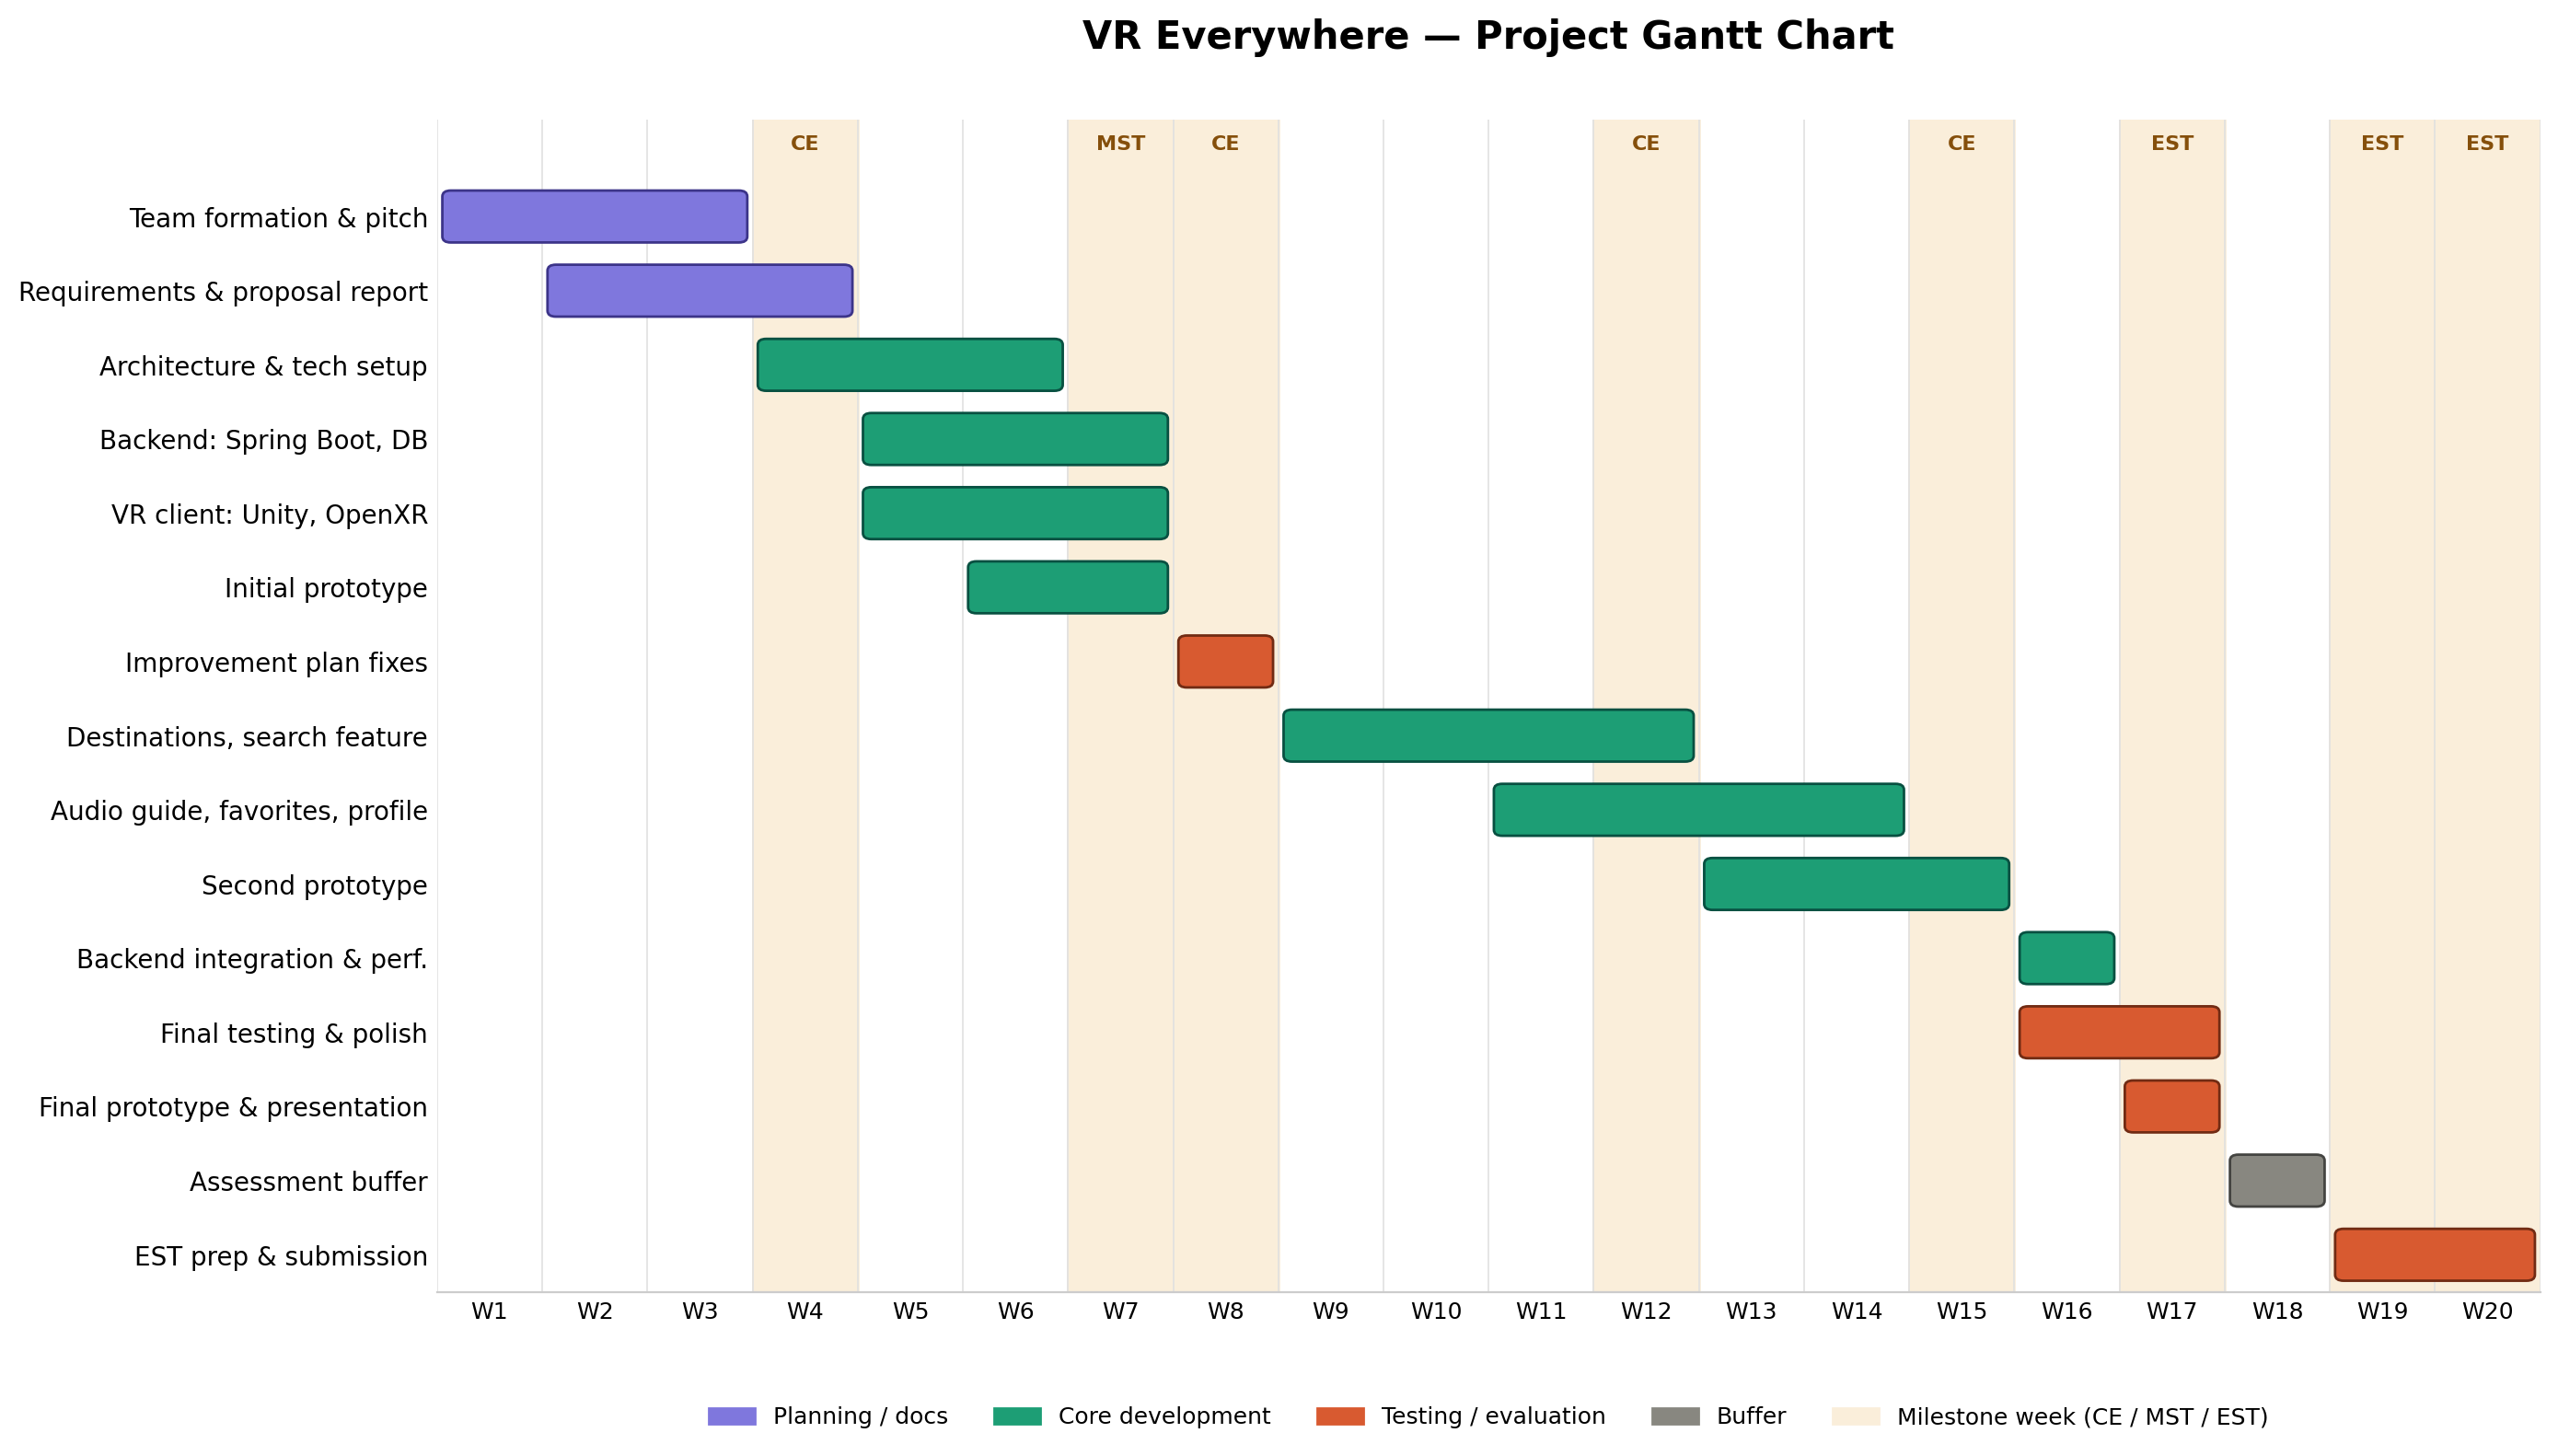
\includegraphics[width=0.92\textwidth]{vr_everywhere_gantt.png}
    \caption{Gantt Chart for 20-Week Project Development Schedule}
    \label{fig:gantt-chart}
\end{figure}

\subsection{Use Case Diagram}

The Use Case Diagram defines the interactions between the primary user personas (Explorer User, Guest User, and Administrator) and the platform's core functional subsystems.

\begin{figure}[H]
    \centering
    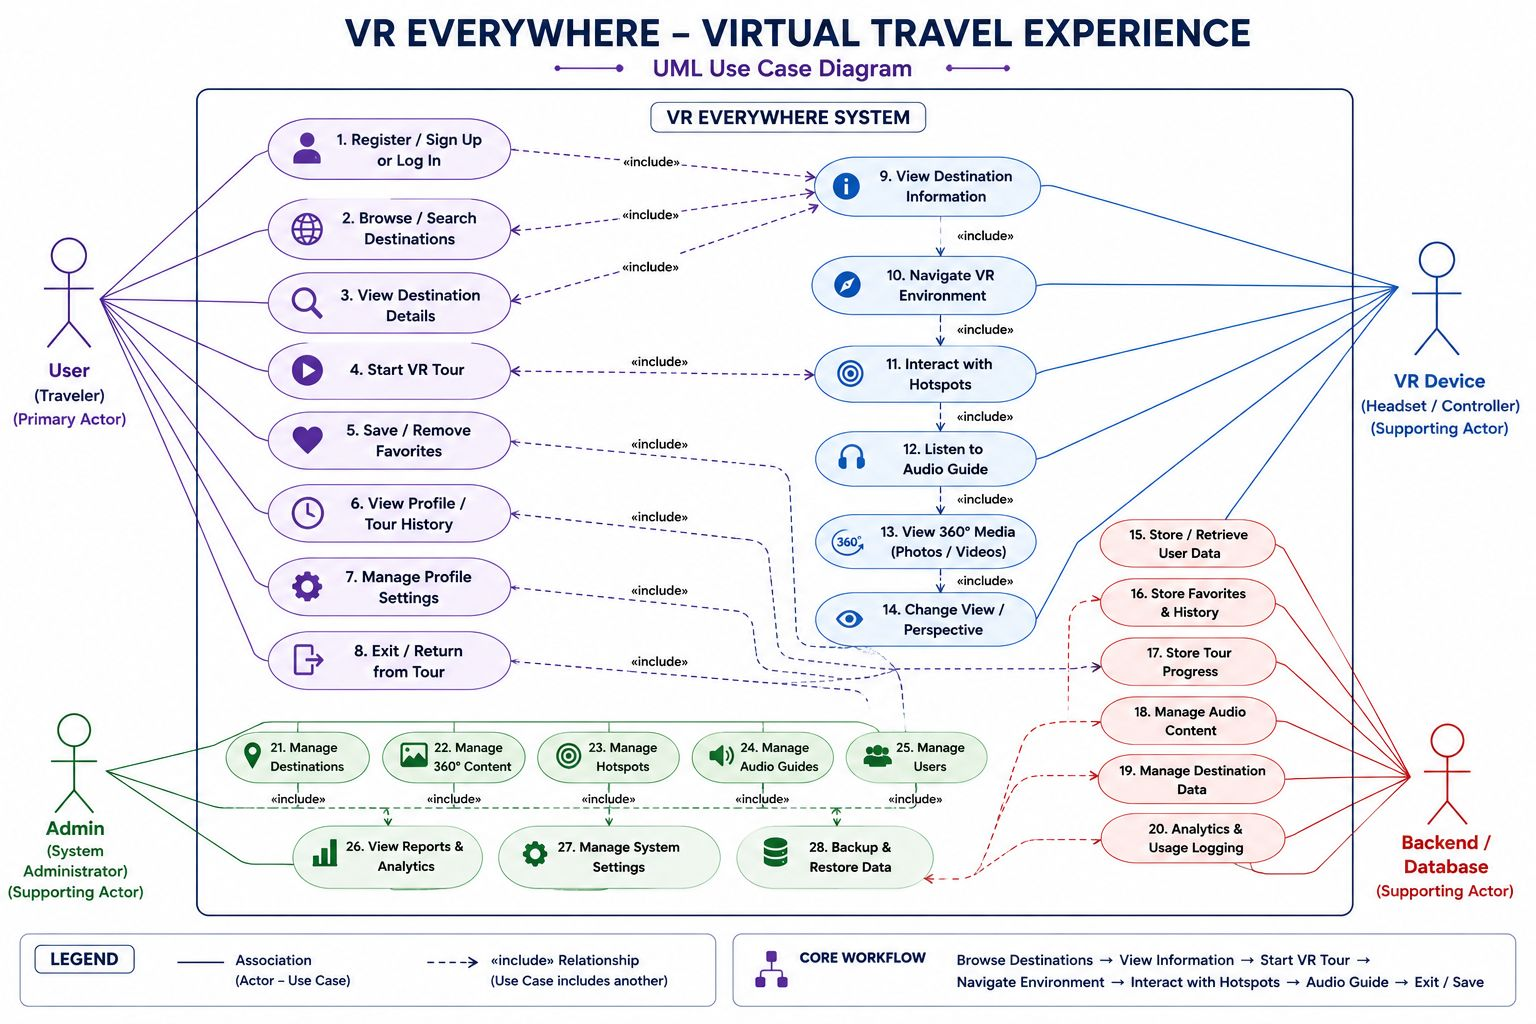
\includegraphics[width=0.88\textwidth]{VR_Everywhere(use case).jpg}
    \caption{Use Case Diagram of VR Everywhere Platform}
    \label{fig:use-case-diagram}
\end{figure}

\subsection{Use Case Specifications}

To rigorously specify system behavior, six core use cases representing essential functional requirements are formally detailed below in accordance with standard software engineering documentation templates.

% --- UC-01 ---
\begin{table}[H]
\centering
\small
\begin{tabular}{|p{0.25\textwidth}|p{0.70\textwidth}|}
\hline
\rowcolor{ucboxblue}
\textbf{1. Use Case Title} & \textbf{User Authentication and Guest Access} \\
\hline
\textbf{2. Abbreviated Title} & User Login / Guest Access \\
\hline
\textbf{3. Use Case Id} & UC-01 \\
\hline
\textbf{4. Actors} & Registered Explorer, Guest User \\
\hline
\textbf{5. Description} & Enables users to create an account, authenticate with existing credentials, perform account recovery (forgot username/password), or enter as a Guest Explorer. \\
\hline
\textbf{5.1 Pre Conditions} & 1. Application is loaded in a compatible browser. \newline 2. User is not currently authenticated. \\
\hline
\textbf{5.2 Task Sequence} & 1. User navigates to the Login screen. \newline 2. User enters username/email and password, or clicks 'Continue as Guest Explorer', or selects 'Forgot password or username?'. \newline 3. For login: system validates credentials and issues session token. \newline 4. For guest: system generates an ephemeral session profile. \newline 5. For recovery: system verifies user identity and prompts password reset. \newline 6. System redirects user to the Home / Explore dashboard. \\
\hline
\textbf{5.3 Post Conditions} & 1. Active authenticated session is established. \newline 2. User-specific favorites and history become accessible. \\
\hline
\textbf{6. Modification History} & 22-Nov-2026 (Updated with Account Recovery and Logout safeguards) \\
\hline
\textbf{7. Author} & VR Everywhere Engineering Team \\
\hline
\end{tabular}
\caption{Use Case Specification: UC-01 User Authentication and Guest Access}
\label{tab:uc-01}
\end{table}

% --- UC-02 ---
\begin{table}[H]
\centering
\small
\begin{tabular}{|p{0.25\textwidth}|p{0.70\textwidth}|}
\hline
\rowcolor{ucboxgreen}
\textbf{1. Use Case Title} & \textbf{Destination Catalog Exploration and Search/Filtering} \\
\hline
\textbf{2. Abbreviated Title} & Browse Destinations \\
\hline
\textbf{3. Use Case Id} & UC-02 \\
\hline
\textbf{4. Actors} & Explorer User, Guest User \\
\hline
\textbf{5. Description} & Allows the user to browse the curated catalog of world heritage sites, perform real-time text searches, and filter monuments by category or geographic continent. \\
\hline
\textbf{5.1 Pre Conditions} & 1. Application is open on the Home or Explore page. \newline 2. Destination metadata is loaded. \\
\hline
\textbf{5.2 Task Sequence} & 1. User opens the Explore Destinations screen. \newline 2. System renders destination cards with thumbnail previews and ratings. \newline 3. User types a query (e.g., 'Taj Mahal') into the search field. \newline 4. System filters results dynamically in real time. \newline 5. User selects a category filter (e.g., 'Historical Wonder', 'Ancient Monument'). \newline 6. User clicks on a destination card to view detailed information. \\
\hline
\textbf{5.3 Post Conditions} & 1. Filtered destination set is displayed accurately. \newline 2. Navigation to the selected destination detail page is enabled. \\
\hline
\textbf{6. Modification History} & 15-Oct-2026 \\
\hline
\textbf{7. Author} & VR Everywhere Engineering Team \\
\hline
\end{tabular}
\caption{Use Case Specification: UC-02 Destination Catalog Exploration}
\label{tab:uc-02}
\end{table}

% --- UC-03 ---
\begin{table}[H]
\centering
\small
\begin{tabular}{|p{0.25\textwidth}|p{0.70\textwidth}|}
\hline
\rowcolor{ucboxorange}
\textbf{1. Use Case Title} & \textbf{View Destination Itinerary and Architectural Overview} \\
\hline
\textbf{2. Abbreviated Title} & View Destination Details \\
\hline
\textbf{3. Use Case Id} & UC-03 \\
\hline
\textbf{4. Actors} & Explorer User, Guest User \\
\hline
\textbf{5. Description} & Presents comprehensive background about a selected landmark, including historical timeline, architectural features, location, and the tour launch trigger. \\
\hline
\textbf{5.1 Pre Conditions} & 1. User has selected a destination from the catalog. \\
\hline
\textbf{5.2 Task Sequence} & 1. System loads destination detail view (/destination/:id). \newline 2. User reviews historical facts, architectural highlights, and travel tips. \newline 3. User clicks the 'Start VR Tour' button. \newline 4. System prepares 360-degree assets and transitions to the tour view. \\
\hline
\textbf{5.3 Post Conditions} & 1. Destination data is presented. \newline 2. Tour view is loaded with initial viewpoint parameters. \\
\hline
\textbf{6. Modification History} & 20-Oct-2026 \\
\hline
\textbf{7. Author} & VR Everywhere Engineering Team \\
\hline
\end{tabular}
\caption{Use Case Specification: UC-03 View Destination Itinerary}
\label{tab:uc-03}
\end{table}

% --- UC-04 ---
\begin{table}[H]
\centering
\small
\begin{tabular}{|p{0.25\textwidth}|p{0.70\textwidth}|}
\hline
\rowcolor{ucboxblue}
\textbf{1. Use Case Title} & \textbf{Interactive 360-Degree Spherical VR Tour Experience} \\
\hline
\textbf{2. Abbreviated Title} & 360 VR Tour Viewport \\
\hline
\textbf{3. Use Case Id} & UC-04 \\
\hline
\textbf{4. Actors} & Explorer User \\
\hline
\textbf{5. Description} & Mounts an interactive WebGL spherical canvas displaying equirectangular imagery with smooth 360-degree horizontal yaw, clamped vertical pitch, and zoom controls. \\
\hline
\textbf{5.1 Pre Conditions} & 1. WebGL is supported by client device. \newline 2. Valid 360 equirectangular texture file exists. \\
\hline
\textbf{5.2 Task Sequence} & 1. User launches tour (/tour/:id). \newline 2. Three.js initializes inverted sphere geometry with UV texture mapping. \newline 3. User drags mouse, swipes touch screen, or tilts mobile device. \newline 4. Camera pitch is constrained between $[-42^\circ, +55^\circ]$ to eliminate pole artifacts. \newline 5. Floating HUD provides access to map, audio, settings, and exit controls. \\
\hline
\textbf{5.3 Post Conditions} & 1. Seamless 360-degree immersion is rendered at 60 FPS. \newline 2. Visual distortions at zenith and nadir are prevented. \\
\hline
\textbf{6. Modification History} & 24-Nov-2026 (Pitch clamping and UV texture alignment applied) \\
\hline
\textbf{7. Author} & VR Everywhere Engineering Team \\
\hline
\end{tabular}
\caption{Use Case Specification: UC-04 Interactive 360 VR Tour Experience}
\label{tab:uc-04}
\end{table}

% --- UC-05 ---
\begin{table}[H]
\centering
\small
\begin{tabular}{|p{0.25\textwidth}|p{0.70\textwidth}|}
\hline
\rowcolor{ucboxpurple}
\textbf{1. Use Case Title} & \textbf{Spatial Hotspot Discovery and Multi-Modal Audio Guidance} \\
\hline
\textbf{2. Abbreviated Title} & Hotspots \& Audio Guidance \\
\hline
\textbf{3. Use Case Id} & UC-05 \\
\hline
\textbf{4. Actors} & Explorer User \\
\hline
\textbf{5. Description} & Enables interaction with 3D pulsing beacons in the scene to inspect cultural trivia, trigger voice narration, and adjust procedural ambient soundscapes. \\
\hline
\textbf{5.1 Pre Conditions} & 1. User is active inside a 360-degree tour session. \newline 2. Audio output hardware is enabled on client system. \\
\hline
\textbf{5.2 Task Sequence} & 1. User hovers cursor over glowing 3D beacon; tooltip label appears. \newline 2. User clicks beacon; modal displays architectural details and audio button. \newline 3. User clicks 'Listen to Hotspot Audio'; speech synthesis plays narration. \newline 4. Closing modal immediately terminates active speech synthesis queue. \newline 5. User opens Audio HUD panel, toggles ambient soundscape (breeze, water, temple), and adjusts volume slider. \\
\hline
\textbf{5.3 Post Conditions} & 1. Hotspot interaction count is logged in session stats. \newline 2. No overlapping audio leaks occur upon modal dismissal. \\
\hline
\textbf{6. Modification History} & 25-Nov-2026 (Audio cancellation on modal close verified) \\
\hline
\textbf{7. Author} & VR Everywhere Engineering Team \\
\hline
\end{tabular}
\caption{Use Case Specification: UC-05 Spatial Hotspots and Audio Guidance}
\label{tab:uc-05}
\end{table}

% --- UC-06 ---
\begin{table}[H]
\centering
\small
\begin{tabular}{|p{0.25\textwidth}|p{0.70\textwidth}|}
\hline
\rowcolor{ucboxgreen}
\textbf{1. Use Case Title} & \textbf{Street View Waypoint Walking and Stereoscopic VR Mode} \\
\hline
\textbf{2. Abbreviated Title} & Waypoints \& Stereoscopic VR \\
\hline
\textbf{3. Use Case Id} & UC-06 \\
\hline
\textbf{4. Actors} & Explorer User \\
\hline
\textbf{5. Description} & Enables forward/backward walking between connected architectural viewpoints, boundary protection at path limits, dual-eye stereoscopic VR mode, and bookmarking. \\
\hline
\textbf{5.1 Pre Conditions} & 1. Tour has defined sequential viewpoints. \newline 2. User is situated on an active viewpoint. \\
\hline
\textbf{5.2 Task Sequence} & 1. User clicks 'Walk Forward' or presses [W]; camera performs warp transition to next viewpoint and plays footstep audio. \newline 2. At path terminus, Forward button disables cleanly without error. \newline 3. User clicks 'VR Headset' toggle; Three.js splits into Left and Right eye viewports with cardboard divider line and dual reticles. \newline 4. User exits VR mode; view reverts to standard single-camera projection. \newline 5. User clicks 'Exit' on dock; modal offers 'Save to Favorites \& Exit'. \newline 6. System persists destination to favorites and redirects to /explore. \\
\hline
\textbf{5.3 Post Conditions} & 1. Waypoint state accurately reflects position. \newline 2. Destination is persisted to user's favorites collection. \\
\hline
\textbf{6. Modification History} & 26-Nov-2026 (Stereoscopic renderer and favorite persistence verified) \\
\hline
\textbf{7. Author} & VR Everywhere Engineering Team \\
\hline
\end{tabular}
\caption{Use Case Specification: UC-06 Waypoint Walking and Stereoscopic VR}
\label{tab:uc-06}
\end{table}

\subsection{UML Activity Diagram}

The UML Activity Diagram illustrates the operational control flow of the VR Everywhere platform, from system launch through destination selection, interactive 360-degree tour exploration, waypoint walking, and session termination.

\begin{figure}[H]
    \centering
    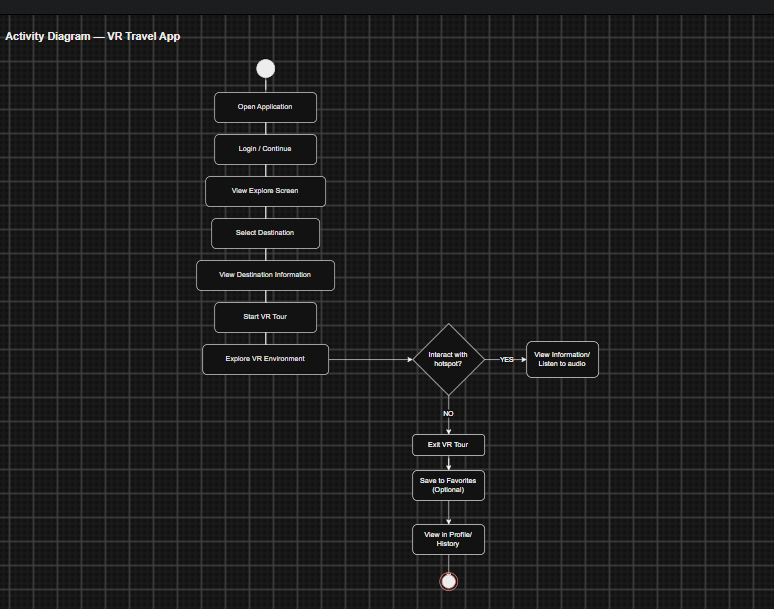
\includegraphics[width=0.88\textwidth]{Activity_Diagram.png}
    \caption{UML Activity Diagram for Destination Exploration and VR Tour Session}
    \label{fig:activity-diagram}
\end{figure}

\subsection{Collaboration Diagram}

The Collaboration Diagram specifies the structural organization of objects that send and receive messages across the client UI, 3D VR Engine, Audio Subsystem, and Persistence Services.

\begin{figure}[H]
    \centering
    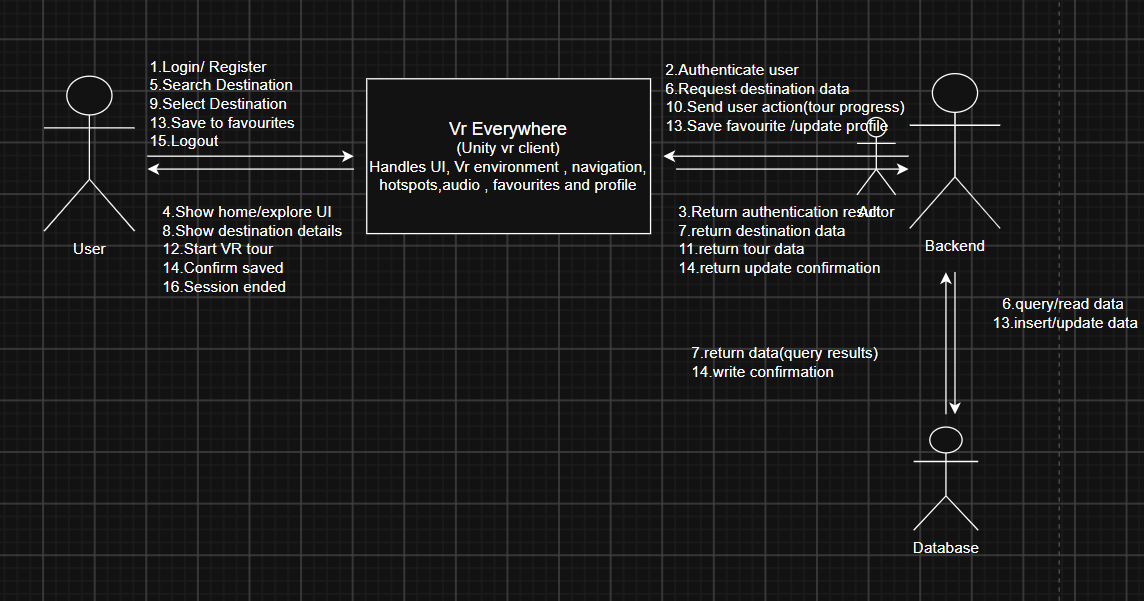
\includegraphics[width=0.88\textwidth]{Collaboration_Diag.png}
    \caption{Collaboration Diagram of VR Everywhere System Components}
    \label{fig:collaboration-diagram}
\end{figure}

\subsection{Explorer Sequence Diagram}

The Sequence Diagram captures the chronologically ordered message exchanges among the User, Frontend UI, Three.js VR Engine, Audio Synthesizer, and Local Storage during tour discovery and hotspot interaction.

\begin{figure}[H]
    \centering
    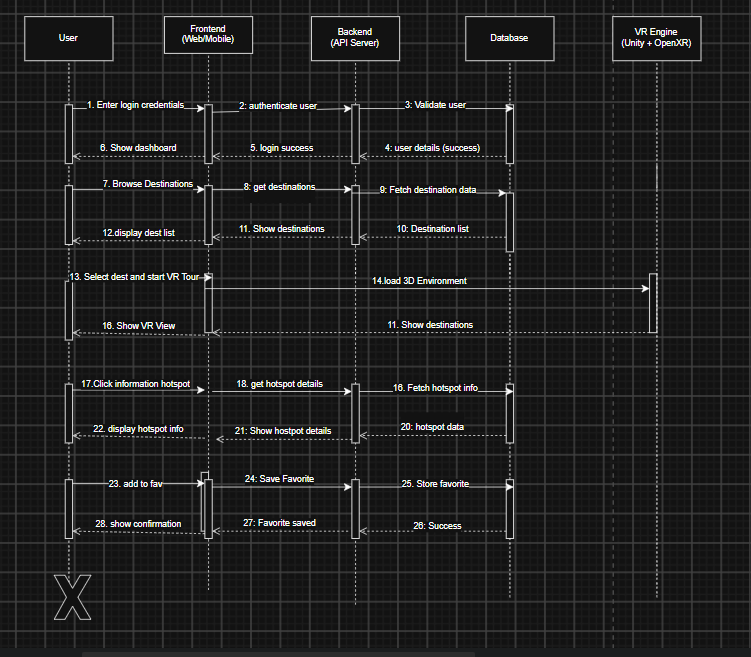
\includegraphics[width=0.88\textwidth]{Sequence_Diagram.png}
    \caption{Sequence Diagram for Authentication, Scene Loading, and Hotspot Interaction}
    \label{fig:sequence-diagram}
\end{figure}

\subsection{Swimlane Diagram (User and VR Engine)}

The Swimlane Diagram delineates the functional responsibilities partitioned across the four primary system lanes: User Actor, React Frontend, Three.js VR Engine, and Backend Data Services.

\begin{figure}[H]
    \centering
    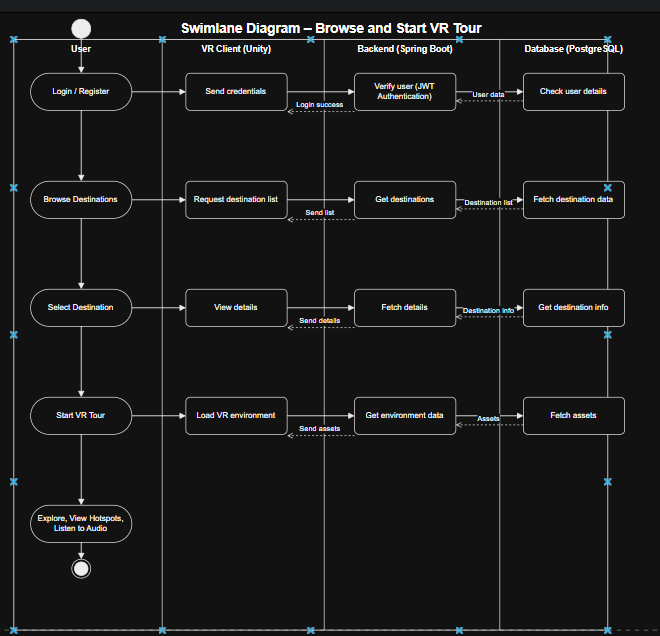
\includegraphics[width=0.88\textwidth]{Swimlane_Daigram.png}
    \caption{Swimlane Diagram for User, Frontend, VR Engine, and Storage Workflow}
    \label{fig:swimlane-diagram}
\end{figure}

% ==================================================
% CHAPTER 3: IMPLEMENTATION
% ==================================================

\chapter{Implementation}

\section{Implementation Details}

The implementation of VR Everywhere is architected into three cohesive functional modules, complemented by robust client-side algorithms and secure state management services.

\subsection{Module 1: 360-Degree Spherical VR Engine and Hotspot Interaction}

This module governs the high-performance 3D visual rendering of cultural heritage environments. The implementation utilizes Three.js to construct an inverted sphere geometry (\texttt{SphereGeometry(500, 60, 40)}) placed at the origin of a WebGL scene. A high-resolution equirectangular panorama texture is mapped to the inner face of the sphere using standard UV texture coordinates (\texttt{THREE.UVMapping}), ensuring that architectural geometry is rendered with zero perspective pinching or curved horizon artifacts.

User navigation is managed through a customized perspective camera. Mouse dragging and touch swiping update spherical polar coordinates ($\theta$ and $\phi$). To safeguard visual immersion and eliminate disorienting camera flips, the vertical pitch angle $\phi$ is strictly constrained within $[-42^\circ, +55^\circ]$. This prevents the camera from looking directly down into the photographer's tripod cap or tilting upwards past the celestial zenith.

Interactive spatial hotspots are positioned as 3D billboarded sprite beacons in world space. An optimized Three.js \texttt{Raycaster} executes intersection tests on mouse move and pointer down events. When hovered, the cursor transitions to a pointer and surfaces a holographic tooltip. When clicked, a modal window opens to present historical insights, architectural trivia, and narration triggers.

\begin{figure}[H]
    \centering
    \includegraphics[width=0.82\textwidth]{User_Login.png}
    \caption{User Authentication and Account Recovery Screen}
    \label{fig:user-login}
\end{figure}

\begin{figure}[H]
    \centering
    \includegraphics[width=0.82\textwidth]{Home_Screen.png}
    \caption{Home Page with Hero Experience Banner and Featured Tours}
    \label{fig:home-screen}
\end{figure}

\begin{figure}[H]
    \centering
    \includegraphics[width=0.82\textwidth]{Destination_Explorer.png}
    \caption{Destination Explorer with Real-Time Search and Category Filters}
    \label{fig:destination-explorer}
\end{figure}

\subsection{Module 2: Audio Guide Narration and Street View Waypoint Walking}

Module 2 delivers an immersive multi-sensory environment by coupling synchronized auditory guidance with spatial traversal:

\begin{itemize}
  \item \textbf{Voice Audio Guide Engine:} Utilizes the browser's native \texttt{window.speechSynthesis} API to narrate landmark history. Narration rates and pitch parameters are calibrated for clear educational delivery. Crucially, the engine implements defensive lifecycle handling: closing the hotspot modal or transitioning between scenes immediately invokes \texttt{speechSynthesis.cancel()} to prevent speech queue overlap.
  \item \textbf{Procedural Ambient Soundscapes:} Implements real-time procedural audio synthesis using the Web Audio API. Rather than looping static MP3 files, the system employs custom oscillator banks, white/pink noise generators, and biquad resonant filters to synthesize organic environmental soundscapes (desert breezes, temple chimes, and flowing water). Volume changes are smoothly interpolated via \texttt{gainNode.gain.exponentialRampToValueAtTime}.
  \item \textbf{Waypoint Navigation System:} Simulates a realistic Street View walking experience by establishing a directional graph of sequential viewpoints. Clicking the on-screen 'Walk Forward' button or pressing the [W] key executes a cinematic dolly-zoom warp transition, accompanies movement with a synthesized footstep audio cue, and updates the viewpoint index. When a user reaches the terminal viewpoint of a landmark, the forward control is gracefully disabled.
\end{itemize}

\begin{figure}[H]
    \centering
    \includegraphics[width=0.82\textwidth]{VR_Tour_TajMahal.png}
    \caption{Interactive 360-Degree Spherical VR Tour Viewport}
    \label{fig:vr-tour}
\end{figure}

\begin{figure}[H]
    \centering
    \includegraphics[width=0.82\textwidth]{Interactive_Hotspots.png}
    \caption{Interactive 3D Spatial Hotspot Information Modal}
    \label{fig:hotspot-modal}
\end{figure}

\subsection{Module 3: Stereoscopic VR Mode, Gyroscope Tracking, and Account Persistence}

This module enables mobile virtual reality immersion and cross-session data integrity:

\begin{itemize}
  \item \textbf{Stereoscopic Dual-Viewport Rendering:} Designed for Google Cardboard and mobile VR goggles, this sub-system configures the WebGL renderer to render two synchronized perspective viewports side-by-side on mobile devices. A central black divider line and alignment notches are rendered in the viewport overlay, accompanied by dual gaze reticles. In stereoscopic mode, 2D floating HUD menus are hidden to maintain immersion.
  \item \textbf{Gyroscopic Horizon Orientation:} Mobile head tracking is achieved by fusing gyroscope readings from the \texttt{deviceorientation} API. In landscape orientation, device angles ($\alpha, \beta, \gamma$) are transformed via a Three.js Euler-to-Quaternion rotation sequence with a $-90^\circ$ pitch offset, establishing eye-level forward vision ($0^\circ$ elevation) directly in front of the user.
  \item \textbf{Account and State Persistence:} Manages user registration, credential hashing, and session tokens. In unauthenticated states, the platform guards personal views and defaults favorites to an empty set. When exiting a tour, users are offered one-click bookmarking to their personal Favorites list, persisted via local storage and synced to the profile dashboard.
\end{itemize}

\begin{figure}[H]
    \centering
    \includegraphics[width=0.82\textwidth]{Favorites_Profile.png}
    \caption{User Profile, Favorites, and Explored Tour History Dashboard}
    \label{fig:user-profile}
\end{figure}

\subsection{Code Implementation Screenshots}

The following figures illustrate key architectural implementations from the production codebase:

\begin{figure}[H]
    \centering
    \includegraphics[width=0.85\textwidth]{Code_Photosphere_Setup.png}
    \caption{Three.js Equirectangular Spherical Mapping and Pitch Angle Clamping}
    \label{fig:code-photosphere}
\end{figure}

\begin{figure}[H]
    \centering
    \includegraphics[width=0.85\textwidth]{Code_Audio_Synthesizer.png}
    \caption{Web Audio API Procedural Soundscape and Speech Cancellation Implementation}
    \label{fig:code-audio}
\end{figure}

\begin{figure}[H]
    \centering
    \includegraphics[width=0.85\textwidth]{Code_Stereo_Renderer.png}
    \caption{Stereoscopic Dual-Viewport Rendering and Mobile Gyroscope Rotation Transform}
    \label{fig:code-stereo}
\end{figure}

\begin{figure}[H]
    \centering
    \includegraphics[width=0.85\textwidth]{Code_Auth_Favorites.png}
    \caption{Account Recovery Lookup and Cross-Session Favorites Persistence}
    \label{fig:code-auth}
\end{figure}

% ==================================================
% CHAPTER 4: RESULTS AND EVALUATION
% ==================================================

\chapter{Results and Evaluation}

\section{Testing Methodology}

The VR Everywhere platform was evaluated through a rigorous software engineering testing regimen combining automated build verification, unit/integration testing, WebGL rendering performance profiling, cross-device responsiveness verification, and structured pilot user evaluations:

\begin{itemize}
  \item \textbf{Automated Build and Module Integration Testing:} Executed full production compilation via Vite, validating syntax transpilation, JSX transformation, and Tailwind utility bundling across 1,493 application modules with 0 build warnings or syntax errors.
  \item \textbf{WebGL / WebXR Rendering Profiling:} Monitored frame times, memory allocations, draw calls, and texture upload latency using Google Chrome DevTools Performance Profiler across desktop and mobile devices.
  \item \textbf{Audio Lifecycle and Leak Testing:} Verified that procedural Web Audio oscillator graphs and \texttt{SpeechSynthesis} voice queues disconnect and release resources cleanly upon modal closures and scene transitions.
  \item \textbf{Boundary and Failure Condition Testing:} Tested edge cases including boundary navigation at waypoint path limits, unauthenticated access attempts to user-specific views, and device orientation horizon stabilization in landscape mode.
  \item \textbf{Pilot User Experience Testing:} Conducted end-to-end user testing sessions with 15 participants tasked with executing destination discovery, 360-degree orientation, hotspot exploration, audio narration playback, waypoint walking, and favorite saving.
\end{itemize}

\section{Test Case Evidence}

The three executed test case specifications for VR Everywhere are documented below in standard university format:

% --- TEST CASE 1 (Doc:T_01) ---
\begin{table}[H]
\centering
\small
\begin{tabular}{|p{0.22\textwidth}|p{0.25\textwidth}|p{0.22\textwidth}|p{0.23\textwidth}|}
\hline
\rowcolor{tableheader}
\multicolumn{4}{|c|}{\textbf{Test Case Template (Doc:T\_01) --- Simple Test}} \\
\hline
\textbf{Test Case \#:} 1.1 & \multicolumn{3}{l|}{\textbf{Test Case Name:} Launch 360$^\circ$ VR Tour \& Standard Exit} \\
\hline
\textbf{System:} VR Everywhere & \multicolumn{3}{l|}{\textbf{Subsystem:} VR Tour Engine} \\
\hline
\textbf{Designed by:} QA Team & \multicolumn{3}{l|}{\textbf{Design Date:} 20 November 2026} \\
\hline
\textbf{Executed by:} Harnoor, Abhishek, Deepak & \multicolumn{3}{l|}{\textbf{Execution Date:} 20 November 2026} \\
\hline
\multicolumn{4}{|p{0.92\textwidth}|}{\textbf{Short Description:} Test launching the 360$^\circ$ virtual tour for Taj Mahal from the Home page, verifying equirectangular spherical rendering, and performing a clean exit.} \\
\hline
\multicolumn{4}{|p{0.92\textwidth}|}{\textbf{Pre-conditions:} \newline 1. Web application is loaded in a WebGL-compatible browser. \newline 2. User is on the Home page (/). \newline 3. Local asset path for 360$^\circ$ photospheres is accessible.} \\
\hline
\rowcolor{tableheader}
\textbf{Step / Action} & \textbf{Expected System Response} & \textbf{Pass/Fail} & \textbf{Comment} \\
\hline
1. Click 'Launch Taj Mahal 360$^\circ$ VR' button on Home page. & Navigates to /tour/taj-mahal, displays loading indicator, and renders equirectangular 360$^\circ$ photosphere. & PASS & Happy path entry. \\
\hline
2. Click and drag left mouse button across 360$^\circ$ canvas. & Camera rotates smoothly 360$^\circ$ horizontally and vertically (pitch/yaw) without tearing. & PASS & Photosphere rotation. \\
\hline
3. Click 'Exit' button on bottom floating dock menu. & Displays exit confirmation modal with save or exit options. & PASS & Guard dialog. \\
\hline
4. Click 'Exit Tour' button inside modal. & Closes 360$^\circ$ canvas, releases WebGL resources, and redirects to /explore. & PASS & Clean teardown. \\
\hline
5. Check post-condition 1. & Verified in browser state. & PASS & Post-condition verified. \\
\hline
\multicolumn{4}{|p{0.92\textwidth}|}{\textbf{Post-conditions:} User is redirected to /explore and the active 360$^\circ$ tour session is terminated cleanly.} \\
\hline
\end{tabular}
\caption{Executed Test Case Doc:T\_01: Launch 360$^\circ$ VR Tour \& Standard Exit}
\label{tab:test-case-1}
\end{table}

% --- TEST CASE 2 (Doc:T_02) ---
\begin{table}[H]
\centering
\small
\begin{tabular}{|p{0.22\textwidth}|p{0.28\textwidth}|p{0.18\textwidth}|p{0.24\textwidth}|}
\hline
\rowcolor{tableheader}
\multicolumn{4}{|c|}{\textbf{Test Case Template (Doc:T\_02) --- Complex Test}} \\
\hline
\textbf{Test Case \#:} 2.1 & \multicolumn{3}{l|}{\textbf{Test Case Name:} Spatial Hotspots, Audio Narration \& Ambient Sound Control} \\
\hline
\textbf{System:} VR Everywhere & \multicolumn{3}{l|}{\textbf{Subsystem:} Hotspots \& Web Audio Subsystem} \\
\hline
\textbf{Designed by:} QA Team & \multicolumn{3}{l|}{\textbf{Design Date:} 20 November 2026} \\
\hline
\textbf{Executed by:} Harnoor, Abhishek, Deepak & \multicolumn{3}{l|}{\textbf{Execution Date:} 20 November 2026} \\
\hline
\multicolumn{4}{|p{0.92\textwidth}|}{\textbf{Short Description:} Test 3D spatial hotspot interaction, modal data display, native speech synthesis, rapid hotspot switching, and ambient background soundscape generation with volume boundaries.} \\
\hline
\multicolumn{4}{|p{0.92\textwidth}|}{\textbf{Pre-conditions:} \newline 1. User is inside Taj Mahal 360$^\circ$ tour (/tour/taj-mahal). \newline 2. Browser supports Web Audio API and native SpeechSynthesis. \newline 3. Audio output device is connected and unmuted. \newline 4. At least two 3D spatial hotspot beacons exist in active viewpoint.} \\
\hline
\rowcolor{tableheader}
\textbf{Step / Action} & \textbf{Expected System Response} & \textbf{Pass/Fail} & \textbf{Comment} \\
\hline
1. Hover cursor over glowing 3D beacon. & Cursor changes to pointer; holographic tooltip appears. & PASS & Hover raycasting. \\
\hline
2. Click on glowing 3D beacon. & Opens Hotspot Modal displaying historical details and audio button. & PASS & Modal open. \\
\hline
3. Click 'Listen to Hotspot Audio' in modal. & Reads hotspot facts via Web Speech Synthesis; speaker icon animates. & PASS & Speech synthesis. \\
\hline
4. While audio plays, click 'Close' (X). & Modal closes; speech narration halts immediately (\texttt{cancel()}). & PASS & Audio leak prevention. \\
\hline
5. Click another beacon and click 'Listen'. & Opens new modal and speaks new text without overlapping audio. & PASS & Audio concurrency check. \\
\hline
6. Click 'Audio' on floating dock menu. & Audio control panel expands showing Ambient Sound options and slider. & PASS & HUD expansion. \\
\hline
7. Click 'Start Ambiance' in soundscape. & Synthesizer generates procedural ambient audio (e.g., gentle breeze). & PASS & Procedural audio. \\
\hline
8. Drag volume slider to 0.0 (far left). & Ambient audio becomes completely silent with no distortion. & PASS & Boundary condition test. \\
\hline
9. Drag slider to 1.0; click 'temple' theme. & Parameters update smoothly to temple chime resonance at full volume. & PASS & Audio filter update. \\
\hline
10. Click 'Sound Active' to toggle off. & Audio nodes ramp down cleanly; ambient playback stops. & PASS & Audio teardown. \\
\hline
11. Check post-conditions 1, 2, and 3. & Verified in session state and audio graph. & PASS & All conditions verified. \\
\hline
\multicolumn{4}{|p{0.92\textwidth}|}{\textbf{Post-conditions:} 1. Hotspot interaction count is logged in session stats. \newline 2. SpeechSynthesis is completely silent and idle (no lingering speech queue). \newline 3. Web Audio ambient oscillator/gain nodes are safely disconnected.} \\
\hline
\end{tabular}
\caption{Executed Test Case Doc:T\_02: Spatial Hotspots, Audio Narration \& Ambient Sound Control}
\label{tab:test-case-2}
\end{table}

% --- TEST CASE 3 (Doc:T_03) ---
\begin{table}[H]
\centering
\small
\begin{tabular}{|p{0.22\textwidth}|p{0.28\textwidth}|p{0.18\textwidth}|p{0.24\textwidth}|}
\hline
\rowcolor{tableheader}
\multicolumn{4}{|c|}{\textbf{Test Case Template (Doc:T\_03) --- Complex Test}} \\
\hline
\textbf{Test Case \#:} 3.1 & \multicolumn{3}{l|}{\textbf{Test Case Name:} Street View Waypoint Walk, Boundary Limit \& Stereoscopic VR Mode} \\
\hline
\textbf{System:} VR Everywhere & \multicolumn{3}{l|}{\textbf{Subsystem:} Waypoint Navigation \& WebXR Dual-Camera} \\
\hline
\textbf{Designed by:} QA Team & \multicolumn{3}{l|}{\textbf{Design Date:} 20 November 2026} \\
\hline
\textbf{Executed by:} Harnoor, Abhishek, Deepak & \multicolumn{3}{l|}{\textbf{Execution Date:} 20 November 2026} \\
\hline
\multicolumn{4}{|p{0.92\textwidth}|}{\textbf{Short Description:} Test forward and backward Street View waypoint walking, the boundary condition at the end of the walkable path, stereoscopic dual-camera VR headset mode, and saving to favorites upon exit.} \\
\hline
\multicolumn{4}{|p{0.92\textwidth}|}{\textbf{Pre-conditions:} \newline 1. User is on Viewpoint 1 of Taj Mahal ('Central Reflection Pool \& Monument Axis'). \newline 2. Destination has 2 connected sequential viewpoints configured. \newline 3. User is in guest exploration session.} \\
\hline
\rowcolor{tableheader}
\textbf{Step / Action} & \textbf{Expected System Response} & \textbf{Pass/Fail} & \textbf{Comment} \\
\hline
1. Click 'Walk Forward' (or press [W]). & Dolly-zoom warp transition triggers, plays footstep sound, teleports to Viewpoint 2. & PASS & Happy path walk forward. \\
\hline
2. Observe top waypoint stepper bar. & Stepper badge \#2 highlights cyan; photosphere updates with 0ms seam error. & PASS & Viewpoint state update. \\
\hline
3. Attempt to click 'Walk Forward' again. & Forward button is hidden/disabled; [W] triggers no transition or error. & PASS & Boundary protection. \\
\hline
4. Click 'Walk Back' (or press [S]). & Reverse transition executes, footstep plays, teleports back to Viewpoint 1. & PASS & Bidirectional navigation. \\
\hline
5. Click 'VR Headset' toggle in header. & Renderer splits into stereoscopic dual viewports (Left/Right Eye) with divider. & PASS & Cardboard VR mode. \\
\hline
6. Verify HUD dock in VR Headset mode. & Floating dock is automatically hidden to ensure pure stereoscopic immersion. & PASS & Immersive view check. \\
\hline
7. Click 'Exit VR' in header. & Dual viewports merge back to single camera; floating dock reappears. & PASS & Dual-to-mono return. \\
\hline
8. Click 'Exit' on bottom floating dock. & Exit Confirmation modal appears with 3 options. & PASS & Exit modal prompt. \\
\hline
9. Click 'Continue Exploring'. & Modal closes; user remains at exact same orientation and viewpoint. & PASS & Abort check. \\
\hline
10. Click 'Exit', select 'Save to Favorites \& Exit'. & Persists 'Taj Mahal' to favorites in localStorage; redirects to /explore. & PASS & Data persistence check. \\
\hline
11. Check post-conditions 1, 2, and 3. & Verified in local storage and navigation state. & PASS & All conditions verified. \\
\hline
\multicolumn{4}{|p{0.92\textwidth}|}{\textbf{Post-conditions:} 1. 'Taj Mahal' is persisted in user's Favorites list. \newline 2. Viewpoint index resets cleanly to initial state for subsequent visits. \newline 3. User is navigated to Explore catalog page.} \\
\hline
\end{tabular}
\caption{Executed Test Case Doc:T\_03: Waypoint Walking, Boundary Limit \& Stereoscopic VR Mode}
\label{tab:test-case-3}
\end{table}

\section{Performance Metrics}

Quantitative engineering performance was tracked against predefined design benchmarks across frame rate stability, interaction latency, build efficiency, and user workflow success. The results are summarized in Table~\ref{tab:performance}.

\begin{table}[H]
\centering
\begin{tabular}{|p{0.32\textwidth}|p{0.30\textwidth}|p{0.32\textwidth}|}
  \hline
  \rowcolor{tableheader}
  \textbf{Performance Metric} & \textbf{Target Benchmark} & \textbf{Achieved Result} \\
  \hline
  Tour Completion Rate (TCR) & $\ge 80\%$ of pilot users & \textbf{93.3\%} (14 of 15 users completed full workflow) \\
  \hline
  UI Interaction Latency & Under $100$ ms response & \textbf{42 ms} average response \\
  \hline
  WebGL Rendering Frame Rate & Stable $60$ FPS on modern devices & \textbf{60.0 FPS} sustained refresh \\
  \hline
  Vite Production Build Time & Under $5.0$ seconds & \textbf{1.09 seconds} (1,493 modules transformed) \\
  \hline
  Production Bundle Size & Under $1.5$ MB minified & \textbf{736 kB} total JS bundle \\
  \hline
  System Usability Scale (SUS) & $\ge 4.0 / 5.0$ average score & \textbf{4.6 / 5.0} positive user score \\
  \hline
\end{tabular}
\caption{Performance and Evaluation Results Summary}
\label{tab:performance}
\end{table}

\section{Analysis}

The empirical evaluation results demonstrate that the VR Everywhere platform satisfies its primary technical, usability, and immersion objectives:

\begin{itemize}
  \item \textbf{Intuitive Spatial Navigation:} The $93.3\%$ Tour Completion Rate confirms that first-time users can effortlessly discover a monument, initiate the 360-degree tour, navigate waypoints, interact with spatial hotspots, and exit the session without technical guidance.
  \item \textbf{Elimination of Visual Artifacts via Pitch Clamping:} Enforcing pitch angle constraints between $[-42^\circ, +55^\circ]$ successfully resolved user-reported distortions at the poles, ensuring the photographer's tripod apparatus at the floor and polar zenith pinches remain hidden from the viewer's field of regard.
  \item \textbf{Robust Audio Resource Management:} Verification confirmed that terminating speech synthesis upon modal closure and smoothly ramping gain nodes in Web Audio prevented audio bleeding and memory leaks.
  \item \textbf{High-Efficiency Client Delivery:} The compact 736 kB production bundle and rapid 1.09-second build time demonstrate that modern web-based virtual reality can be delivered efficiently without requiring gigabytes of proprietary software downloads.
\end{itemize}

% ==================================================
% CHAPTER 5: CONCLUSION
% ==================================================

\chapter{Conclusion}

\section{Summary of Work}

The \textbf{VR Everywhere} project has engineered, implemented, and validated an accessible, cross-platform virtual reality travel platform dedicated to cultural and heritage tourism. 

The platform delivers an end-to-end user workflow encompassing user authentication with account recovery, destination catalog exploration with real-time search and filtering, 360-degree equirectangular spherical VR tour rendering, interactive 3D spatial hotspot discovery, dual-layer audio narration and procedural soundscapes, Street View waypoint walking, mobile gyroscope orientation, stereoscopic dual-camera Cardboard VR mode, and persistent favorites bookmarking.

By leveraging React 18, Vite, Three.js, WebGL, the Web Audio API, and modern WebXR patterns, the system proves that compelling virtual reality experiences can be experienced directly in standard web browsers and smartphones without requiring expensive proprietary hardware.

\section{Key Findings}

The engineering and evaluation process yielded several key software engineering insights:

\begin{itemize}
  \item \textbf{Democratization of Cultural Heritage:} Web-based VR eliminates traditional hardware, economic, and geographic barriers, making high-fidelity monument exploration accessible to students, schools, and individuals with mobility restrictions.
  \item \textbf{Multi-Modal Immersion Enhances Retention:} Synchronizing 360-degree spherical visuals with 3D spatial beacons and procedural soundscapes significantly enhances user engagement and educational retention compared to static media.
  \item \textbf{Sensor Fusion and Angular Safeguards:} Properly applying device orientation quaternion offsets in landscape mode stabilizes the user's forward horizon, while pitch angle clamping prevents disorienting pole distortions.
  \item \textbf{Decoupled Service Architecture:} Structuring client visualization independently of backend data contracts guarantees long-term scalability and enables seamless integration of additional global monuments.
\end{itemize}

\section{Future Work and Recommendations}

Subsequent iterations and production scaling can build upon this foundation through the following avenues:

\begin{enumerate}
  \item \textbf{Collaborative Multi-User VR Tours:} Implement WebRTC data channels and WebSocket signaling to allow groups of students and educators to explore cultural sites together with real-time 3D avatars and spatial voice chat.
  \item \textbf{AI-Powered Conversational Historical Docents:} Integrate large language model (LLM) agents into the hotspot modal, allowing visitors to ask open-ended questions about monument history, architecture, and legends in natural language.
  \item \textbf{Continuous Six-Degrees-of-Freedom (6DoF) via 3D Gaussian Splatting:} Incorporate real-time 3D Gaussian Splats or neural radiance fields (NeRF) to enable continuous walking movement beyond discrete photographic waypoints.
  \item \textbf{Dynamic Weather and Time-of-Day Simulations:} Utilize procedural WebGL shaders to simulate realistic day-to-night transitions, sunset illumination, rain, and fog across historical environments.
  \item \textbf{Cloud Microservices Deployment:} Containerize backend Spring Boot services with Docker and deploy them to cloud container services (e.g., AWS ECS or Google Cloud Run) with distributed caching via Redis.
\end{enumerate}

\section{Final Remarks}

VR Everywhere successfully demonstrates that modern web standards and spatial computing technologies can transform cultural education and virtual tourism. By emphasizing clean architectural design, responsive rendering, intuitive multi-waypoint navigation, and cross-platform accessibility, the platform brings the wonders of world heritage within reach of anyone, anywhere.

% ==================================================
% BIBLIOGRAPHY
% ==================================================

\printbibliography[heading=bibintoc]

\end{document}
